\chapter{Introduction and Platform overview}

Data is now at the center of organizations and is increasingly heterogeneous, meaning that there is an explosion of data sources 
that each exposes data in its own format that can be structured, semi-structured or non-structured.
Another major trend is that data processing needs to be real-time, because managers no longer want to wait a whole day 
to have reports and alerts on their business data.
\\

To achieve these requirements, traditional monolithic Data Wharehouse softwares start to be out-dated. They often
propose to deal with only structured data to map it in a relational model, and are often batch-oriented: 
the ETL mechanism (data extraction, transform and load) regularly happen once or twice day, and there is no mechanism 
for real-time subscriptions of new events happening on the data as highlighted by Jay Kreps, principal staff engineer at LinkedIn \footfullcite{bib:linkedinLog}.
\\

The platform I present in this thesis is an event-oriented Data Integration and Stream Processing platform that allows data consumers
to subscribe to data changes in real-time. The main shift from traditional Data Wharehouse softwares is that the whole
system is organized around the notion of \textit{immutable event}. Such a data system captures from various data sources
a historical record of immutable events. Each event represents the change (creation, update or deletion) made to the data at a particular time. 
Based on the Event-Sourcing principle \footfullcite{bib:eventSourcing}, events are stored in a Journal that is an ordered sequence of 
events. Then, the stream of events coming from the Journal can be processed by data consumers that can react to the change of data. 
An example of data consumer can be one that maintain a pre-computed view on the data that is updated upon each event, or one that push 
notification to another service upon a certain kind of events (see Figure \ref{fig:main_archi} for the global architecture).
\\

An example use case is when an organization uses different SaaS services for each of its teams. For instance, the sales
team uses a SaaS software to process their sales pipeline, the project management team uses another SaaS software to manage
the production teams, etc... Without a central data backbone, it is not possible to have a global view on the company data.
The platform I present in this thesis can integrate these different SaaS softwares using their REST API, detect what
changes have been made on the data, and emits the corresponding events. As a result, data consumers can use these events
to update dashboards about the company data in real-time, mixing the data coming from different sources. A data consumer can also push a
notification to SaaS service X when it receives an event from SaaS service Y, allowing real-time synchronization between
heterogeneous services.
\\

An advantage of Event Sourcing is that the whole history of the system is stored. Events are immutable changes made to the data
and are always appended to the Journal (never deleted or modified). As a result, the system stores not only the current state
of the data, but also all its previous states. This allows two interesting properties.

First, it is possible to query past states of the data. This can be very useful for various use cases
where one is interested in the data history, for example a financial audit.

Moreover, storing all the data changes greatly improves the fault-tolerance of the system. As events are not deleted, it is always possible 
to come back in the past in the Journal, delete some delete events that were put by mistake, and replay the events after
them to re-build the system in a right state. This is also referred as Human Fault-Tolerance \footfullcite{bib:human-ft}: in a mutable system,
if an user accidentally delete a data entry, it is lost for ever. But in an immutable system, the deletion is just another
event added to the journal. Figure \ref{fig:event-sourcing} illustrates the difference between a mutable system and an immutable event-sourced system.
\\ 
\begin{figure}[h]
  \begin{center}
    \makebox[\textwidth]{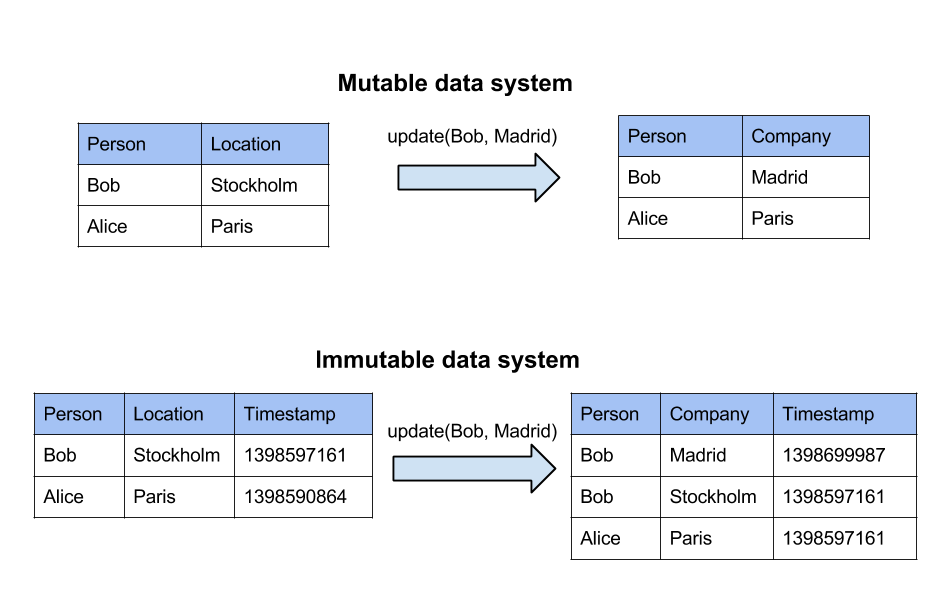
\includegraphics[width=1.0\textwidth]{img/event-sourcing.png}}
    \caption{Immutable datastore and the Event Sourcing principle}
    \label{fig:event-sourcing}
  \end{center}
\end{figure}

This kind of architecture is also known as CQRS \footfullcite{bib:cqrs}. The core principle of CQRS is to decouple the write part and the read part
of a system. The write part (Data Integration) only needs to push immutable events to the Journal in an append-only fashion, which
is very efficient because there is no mutation of the data and no read-write contentions as in traditional databases.
The read part is a set of denormalized pre-computed view that are optimized for low read latency (as the view are automatically re-computed
when a new related event comes in).
An obvious downside of such an architecture is that data is eventually consistent: when a data producer has received the acknowledgment
from the Journal, there is no guarantee that data consumers has already processed the event and updated the data view. However eventual consistency is not
a problem for the functional requirements of the platform.

This model also allows very easy distribution of the platform. Easy distribution because it is a message-oriented
architecture where each component (data producer, journal, data consumers with data views) only exchanges messages (events) to each other (share-nothing architecture).
\\

The platform is composed of three main parts: 
\begin{itemize}
  \item Data Integration, that must integrate several data sources in order to emit 
events (data changes) to the Journal. 
  \item Journal, an abstraction for a sequence of immutable events. The Journal must expose methods to insert events,
  and expose methods to subscribe to the stream of events.
  \item Stream processing, where one can define a tree of data consumers (stream processors) that can react to
  events, maintain derived pre-computed view on the data, and emit new stream of events.
\end{itemize}

\begin{figure}[h]
  \begin{center}
    \makebox[\textwidth]{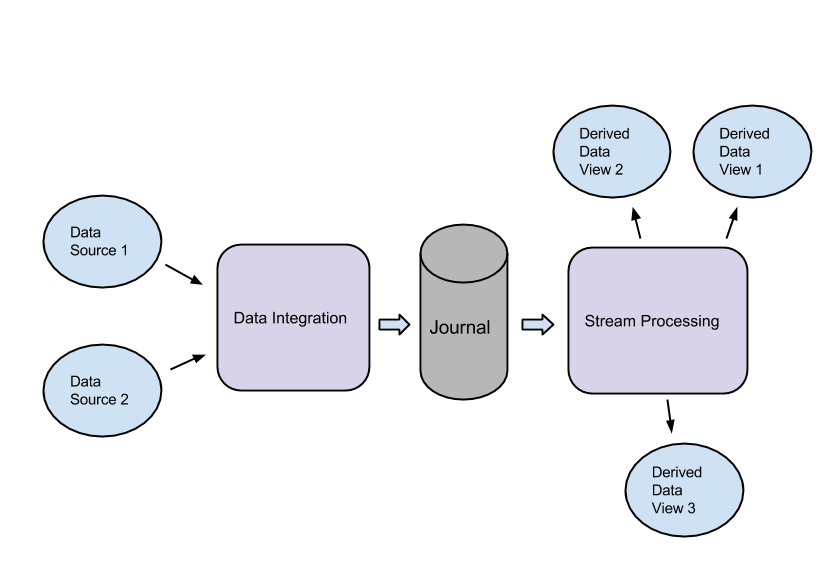
\includegraphics[width=1.0\textwidth]{img/main_archi.png}}
    \caption{Global architecture}
    \label{fig:main_archi}
  \end{center}
\end{figure}

Nonetheless, this kind of evented architecture must be done with a lot of care concerning technical architecture.
The platform needs to do lot of IO in order to push the stream of events from data sources to data consumers, and must
parallelize a lot of operations. Moreover, it must ensure that the stream of events (producers) does not overwhelm the stream
processors (consumers), i.e if consumers process data slowly, producers must try to slow the push rate. The platform should also deal with possible
failure of components and offer strong guarantees on these cases (like no message loss or duplication).

In order to fulfill those requirements, the platform will apply the principles of the Reactive Manifesto \footfullcite{bib:reactiveManifesto} in order to guarantee
that the platform is \textit{scalable, event-driven, resilient and responsive} (the four Reactive Traits). An asynchronous non-blocking approach with a share-nothing architecture will be used to develop the platform in order to optimize resource consumption, decouple components to be able to distribute them easily, take easily advantage of parallelization and handle failures. 
The platform is developed using functional programming in the Scala programming language \footfullcite{bib:scala} in order to leverage functional programming abstractions to better handle asynchronous and stream-oriented code.
\\

